\section{Reconstruction de CFG}
\label{sec:reconstruction}
  
    % Limitation des approches de reconstruction de CFG à partir des fichiers
    % sources et nécessité du fichier exécutable pour la reconstruction de CFG.

    Les instructions machine, ou simplement instructions, sont les opérations de
    base codées en langage machine que peut manipuler un processeur. Un fichier
    exécutable contient l'ensemble des instructions d'un programme. Ce type de
    fichier est généralement produit par la compilation des fichiers sources
    d'un programme écrits dans un langage de haut niveau -- un langage de
    programmation -- vers un langage de bas niveau -- le langage machine.
    
    De manière formelle, un programme $P$ est un sous-ensemble fini de
    $\mathcal{LI}$ avec $\mathcal{LI} = \mathcal{L} \times \mathcal{I}$ un
    ensemble d'instructions étiquetées tel que $\mathcal{L}$ est un ensemble
    fini d'étiquettes ; $\mathcal{I}$ est un ensemble fini d'instructions ;
    $\nexists (l,i),(l',i') \in \mathcal{L} \times \mathcal{I}$ tel que $l =
    l'$.  On note aussi $\mathcal{V}$ l'ensemble des variables de $P$. La figure
    \ref{fig:dump} donne le code désassemblé du fichier binaire exécutable
    \texttt{fibcall-O2.elf}.

    \vspace{1em}
    
    Afin de procéder à une reconstruction précise d'un CFG, et a fortiori d'une
    analyse temporelle précise, il est nécessaire de s'appuyer sur le fichier
    exécutable issu de la compilation des fichiers sources du programme
    considéré et non directement sur les fichiers sources eux-mêmes.

    \vspace{1em}
    
    \begin{figure}[ht]
      \centering
      \begin{subfigure}{.45\textwidth}
        \centering
        \includegraphics[scale=0.45]{img/dump.eps}
        \captionsetup{justification=centering}
        \caption{\emph{dump} de \texttt{fibcall-O2.elf} \\
          $R = \{r1, r3, r8, r9, r10, lr, ctr\}$}
        \label{fig:dump}
      \end{subfigure}
      \begin{subfigure}{.45\textwidth}
        \centering
        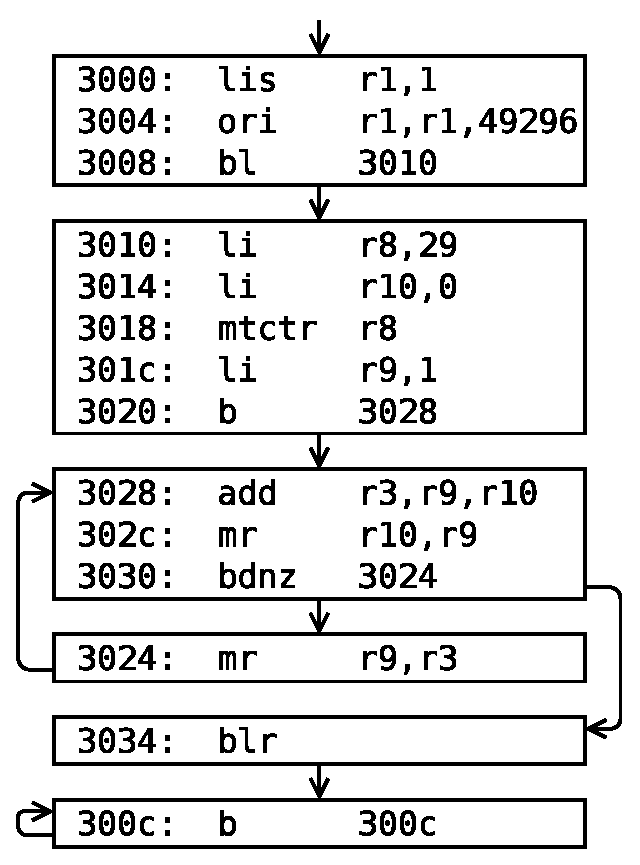
\includegraphics[scale=0.45]{img/recons.eps}
        \captionsetup{justification=centering}
        \caption{CFG de \texttt{fibcall-O2.elf}}
        \label{fig:recons}
      \end{subfigure}
      \caption{Processus de reconstruction d'un CFG}
    \end{figure}

    % Définition de CFG et bloc de base

    Un bloc de base est une séquence d'instructions qui n'a qu'un point
    d'entrée, sa première instruction, et qu'un point de sortie, sa dernière
    instruction.  Le graphe de flot de contrôle d'un programme est un graphe
    orienté dans lequel les noeuds représentent les blocs de base issus du
    programme et les transitions représentent les enchainements possibles entre
    les différents blocs de base lors de l'exécution du programme.

    De manière formelle, un CFG est un tuple $G = (V, E, u, v)$, où les noeuds
    $V$ correspondent aux blocs de bases, les transitions $E \subset V \times V$
    sont les chemins du flot de contrôle, $u \in V$ représente le n{\oe}ud
    d'entrée et $v \in V$ le n{\oe}ud de sortie. La figure \ref{fig:recons}
    donne le CFG reconstruit à partir du fichier binaire exécutable
    \texttt{fibcall-O2.elf}.

    \vspace{1em}
    
    % Principes de recontruction des blocs de base

    Afin de procéder à la reconstruction du CFG d'une tâche, il est tout d'abord
    nécessaire d'en reconstruire les blocs de base. Pour cela il faut identifier
    les points d'entrée de ses différents blocs de base. Une instruction est une
    entrée de bloc de base si elle se trouve être :
    
    \begin{itemize}
      \item le point d'entrée du programme ;
      \item une cible de saut ;
      \item immédiatement après une instruction de saut ;
      \item la première instruction du fichier exécutable.
    \end{itemize}
    
    Les blocs de base sont ensuite construits séquentiellement par accumulation
    des instructions se trouvant entre un point d'entrée de bloc de base inclus
    jusqu'au point d'entrée suivant exclus.
  
    % Principes de recontruction des CFG
    
    Pour reconstruire un CFG il est ensuite nécessaire d'identifier le n{\oe}ud
    d'entrée. C'est le n{\oe}ud correspondant au bloc de base issu du point
    d'entrée du programme. Il faut ensuite en retrouver les transitions. Elles
    sont obtenues itérativement en associant à chaque bloc de base les cibles
    possibles de son point de sortie. Déterminer les cibles possibles d'un bloc
    de base n'est pas une opération triviale, cela s'avère même parfois
    indécidable statiquement.
